\documentclass{article}
\usepackage[margin=2cm]{geometry}
\usepackage{graphicx}
\usepackage[pages=some]{background}
\usepackage{titling}
\usepackage{tabularx}
\usepackage{tikz}
\usepackage{forest}
\usepackage{float}
\usepackage{amsmath}
\usepackage{amssymb}
\usepackage{xcolor}
\usepackage{tcolorbox}

\forestset{
  my box/.style={
    draw,
    rectangle,
    rounded corners,
    fill=gray!20,
    inner sep=6pt,
    minimum width=3cm % Adjust the width as needed
  }
}


\geometry{a4paper}

\backgroundsetup{
    scale=1,
    angle=0,
    opacity=1,
    contents={%
        
\includegraphics[width=\paperwidth,height=\paperheight]{institution_logo.jpg}
    }
}

\newcommand{\subtitle}[1]{
    \posttitle{
        \par\end{center}
        \begin{center}\large#1\end{center}
        \vskip0.5em}
}

\title{ME-421}
\author{Md. Hasibul Islam}
\subtitle{FLUID MACHINERY}

\begin{document}
\begin{titlepage}
    \centering
    
    {\Huge\bfseries\maketitle}
    \textbf{Mohammad Ali Sir} \\
    \vspace{2cm}
    
\includegraphics[width=8cm]{institution_logo.jpg}
    \vfill
    \vspace*{2cm}
\end{titlepage}

\tableofcontents
\pagebreak
\section{Lecture 01: Introduction} 
\hfill Date: 03/06/2023
\subsection*{Booklist}

\textbf{Hydraulic Machines through worked out problems}

\hfill Published by BUET


\section{Lecture 2: Principles of Hydraulic Machinery}
\hfill Date: 05/06/2023

\subsection{Dynamic Action of Fluid}

When a stream of fluid enters a machine, it generally follows a specific direction. However, in order to alter its velocity, either in magnitude or direction, a force must be applied to the fluid. This force, exerted by the motion of the fluid, is referred to as dynamic force. The power of the machine is determined by the dynamic force generated by the flowing fluid, which arises due to the change in momentum.

Momentum can exist in linear or angular form, with angular momentum being the moment of linear momentum. The force is the rate of change of linear momentum, while torque is the rate of change of angular momentum. According to Newton's second law, the rate of change of momentum is proportional to the applied force and occurs in the direction of the force. Specifically, if the resultant external force in the $x$-direction is $F_x$, the mass of the fluid is $m$, the velocity of the fluid is $v_x$, and the change in velocity over time $dt$ is $dv_x$, then:
\\

The change in momentum = $mdv_x$,

And the rate of change of momentum  $= m \frac{dv_x}{dt}$
\begin{equation}
F_x = m \frac{dv_x}{dt} \label{eq:eq1}
\end{equation}

$eq^n$ (\ref{eq:eq1}) is knows as linear momentum $eq^n$.

This $eq^n$ may be wriiten as -
\begin{equation}
F_x dt = mdv_x \label{eq:eq2}
\end{equation}

This $eq^n$ is known as impulse momentum $eq^n$.

For a control volume with fluid entering in uniform velocity $v_{x_{1}}$, and leaving after time $t$ within uniform velocity $v_{x_{2}}$, then according to $eq^n$ (\ref{eq:eq2}),
\begin{equation}
	F_x = \frac{m}{t} (v_{x_{2}}-v_{x_{1}}) \label{eq:eq3}
\end{equation}

Again, $$\frac{m}{t}=\rho Q$$
\begin{equation}
	\Rightarrow F_x = \rho Q (v_{x_{2}}-v_{x_{1}}) \label{eq:eq4}
\end{equation}

Dynamic force exerted by fluid jet on stationary flat plate - 

\subsubsection{Plate normal to jet:}
A fluid jet is issued from a nozzle and strike a flat plate with a velocity $v$. The plate is held stationary at perpendicular to the centerline of the jet. Let,

\begin{center}

$Q \longrightarrow $  Volumetric flow rate\\
$\rho Q \longrightarrow$ Mass flow rate
\end{center}

Dynamic force on the fluid by the plate:
\\
Applying $eq^n$ \ref{eq:eq4}, 
$$F_x = \rho Q (v_{x_{2}} - v_{x_{1}}) $$
$$\Rightarrow -F_x = \rho Q (0-v)$$
\begin{equation}
	\Rightarrow F_x = \rho Q v \label{eq:eq5}
\end{equation}
\begin{equation}
	\Rightarrow F_x = \frac{\gamma}{g} Q v \label{eq:eq6}
\end{equation}

\begin{figure}[H]
  \centering
  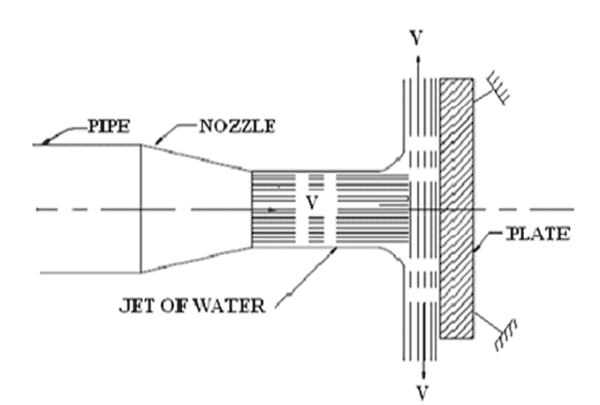
\includegraphics[width=0.75\textwidth]{img/flat_plate.png}
  \caption{Plate normal to jet.}
  \label{fig:Plate normal to jet}
\end{figure}

If $a$ is the area of jet,
$$F_x = \frac{\rho}{g} a v  v$$
\begin{equation}
	\textcolor{red}{\Rightarrow F_x = \frac{\rho}{g} a v^2} \label{eq:eq7}
\end{equation}

\subsubsection{Inclined Plate}
\begin{figure}[H]
  \centering
  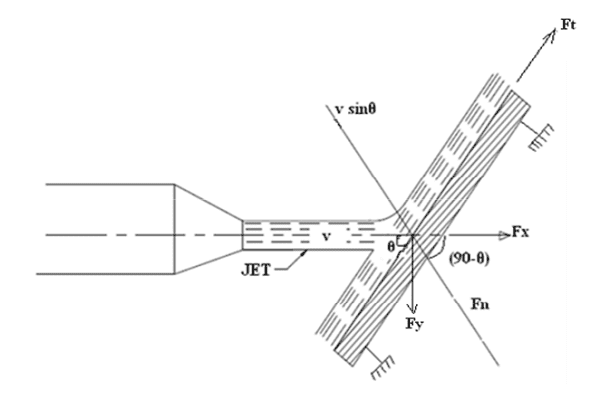
\includegraphics[width=0.75\textwidth]{img/inclined_plate.png}
  \caption{Plate inclined to jet.}
  \label{fig:Plate inclined to jet}
\end{figure}
\vspace{0.25cm}

$$F = F_n = \rho Q v sin\theta $$
Again, $$F_x = F sin\theta$$
$$= (\rho Q v sin \theta) sin \theta $$
\begin{equation}
	\textcolor{red}{F_x = \rho Q v sin^2 \theta} \label{eq:eq8}
\end{equation}
\\
And, $$F_y = F cos\theta$$
\begin{equation}
	\textcolor{red}{\Rightarrow F_y = \rho Q v sin\theta cos\theta} \label{eq:eq9}
\end{equation}
\vspace{0.25cm}
\paragraph*{Determine of division of flows:}
Let $F_s$ ($F_t$ in fig. \ref{fig:Plate inclined to jet}) be the force along the inclined surface of plate and $Q_1$ and $Q_2$ are quantities of flow along the surface. As there is no change in elevation of pressure before and after impact, the magnitude velocity leaving the plate will remain the same. \\
\\
since no force is exerted on the fluid by the plate in "S" direction, then,
\begin{equation}
	F_s = 0 = \rho Q V cos\theta \label{eq:eq10}
\end{equation}
Again, 
\begin{equation}
	\rho Q_1 v - \rho Q_2 v = 0 \label{eq:eq11}
\end{equation}

From $eq^n$ (10) \& (11),
$$\rho Q v cos\theta = \rho Q_1 v - \rho Q_2 v $$
\begin{equation}
	\Rightarrow Q cos\theta = Q_1 - Q_2 \label{eq:eq12}
\end{equation}

From continuity $eq^n$, 
\begin{equation}
	Q_1 + Q_2 = Q \label{eq:eq13}
\end{equation}

From $eq^n$ (12) \& (13),


$$Q_1 = \frac{1}{2} Q (1+cos\theta)$$ 
  \begin{equation}
     Q_2 = \frac{1}{2} Q (1-cos\theta) \label{eq:eq14} 
  \end{equation}

\pagebreak

\section{Lecture 3}
\hfill Date: 12/06/2023

\subsubsection*{Problem}
A jet of water with a velocity of 35 $m/s$ strikes a plat inclined of 30°, cross sectional area if jet 25 $cm^2$. Find the force exerted by the jet on the plate. Calculate the components of force and find the ratio in which the discharge gets divided after striking the plate. 

\subsubsection*{Solution:}
Given, 
\begin{align*}
  \text{velocity, } v &= 35 \, \text{m/s}\\
  \text{angle, } \theta &= 30^\circ \\
  \text{cross-sectional area, } a &= 25 \, \text{cm}^2 \\
  \\
  \text{Volumetric flow rate, } Q &= a \times v \\
  &= 0.0025 \times 35 \, \text{m}^3/\text{s} \\
  &= 0.0875 \, \text{m}^3/\text{s} \\ 
  \\
  \text{Force, } F &= \rho Q v \sin\theta \\
  &= 1000 \times 0.0875 \times 35 \times \sin(30^\circ) = 1531.25 \, \text{N} \\
  \\
  F_x &= F \sin\theta = 765.6 \, \text{N} \\
  F_y &= F \cos\theta = 1326.1 \, \text{N} \\
  \\
  Q_1 &= \frac{Q}{2} (1 + \cos\theta) = 0.0816 \, \text{m}^3/\text{s}\\
  Q_2 &= \frac{Q}{2} (1 - \cos\theta) = 0.00586 \, \text{m}^3/\text{s}\\
  \therefore \frac{Q_1}{Q_2} &= 13.92\\
\end{align*} 

\subsection{Thrust on moving flat plate normal to the direction of jet}
\begin{figure}[H]
  \centering
  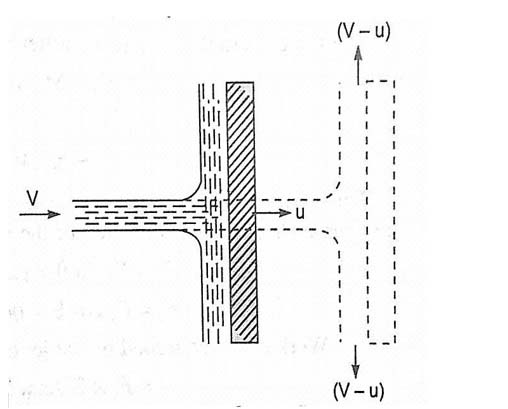
\includegraphics[width=0.5\textwidth]{img/Thrust_on_moving_flat_plate_normal_to_the_direction_of_jet.jpg}
  \caption{Thrust on moving flat plate normal to the direction of jet}
  \label{fig:Thrust_on_moving_flat_plate}
\end{figure}

Let, the flat plate moves with a velocity $u$ in the direction of the jet and the velocity of jet is $v$. The effective velocity with which the jet strike the plate = $v-u$. The mass of the fluid striking the plate per second = $\rho a (v-u)$, where $a$ is the area of the jet. \\
Thrust exerted on the plate in the direction of the jet is, 
\begin{align*}
  F &= \rho a (v-u) [(v-u) - 0]
  % F &= \rho a (v-u)^2
\end{align*}
\begin{equation}
    F = \rho a (v-u)^2 \label{eq:eq15}
\end{equation}

\begin{equation}
    \text{work done per second} = F \times u = \rho a (v-u)^{2} \times u \label{eq:eq16}
\end{equation}

However, this is not practically feasible, because the distance between the nozzle at the plate is go on increasing. If a series of plates were so arranged that each plate appeared successively before the jet in the same position and always moving with a velocity $u$ to the direction of the jet. Then mass of the fluid striking the plate = $\rho a v$.

*note : \textcolor{red}{ [ The whole flow of the nozzle is utilized by the plate. ]}

\begin{figure}[H]
  \centering
  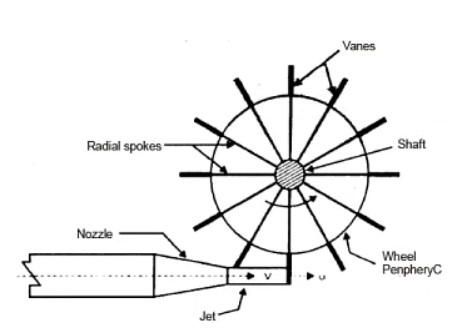
\includegraphics[width=0.5\textwidth]{img/radial_plate.jpg} 
  \caption{Thrust on Successive moving plat normal to the direction of jet}
  \label{fig:Successive_moving_plate}
\end{figure} 


The thrust on the plate,
\begin{align*}
  F &= \rho a v [(v-u) - 0] \\
  &= \rho a v (v-u)\\
\end{align*}

Work done per second = $F \times u$
\begin{equation}
  = \rho a v (v-u) u \label{eq:eq17}
\end{equation}

\begin{align*}
  \text{Now, the input power} &= \text{K.E. of the jet} \\
  &= \frac{1}{2} m v^2 \\
  &= \frac{1}{2} \rho a v \times v^2 
\end{align*}
\begin{equation}
  \therefore \text{Input power} = \frac{1}{2} \rho a v^3 \label{eq:eq18}
\end{equation}

The efficiency of the the wheel,
$$\eta = \frac{\rho a v (v-u) u}{\frac{1}{2} \rho a v^3}$$
\begin{equation}
  \eta = \frac{2u (v-u)}{v^2} \label{eq:eq19}
\end{equation}

\checkmark Generally $u$ is changed, $v$ is not changed significantly.\\

For a given jet velocity, efficiency will be maximum, if,


\begin{align*}
  \frac{d\eta}{du} &= 0 \\
  \frac{d}{du} \left[\frac{2u(v-u)}{v^2}\right] &= 0 \\
  2v - 4u &= 0 \\
  u &= \frac{v}{2}
\end{align*}

For the maximum efficiency of wheel, the peripheral speed of the wheel is equal to half of the jet velocity. \\

The max efficiency is given by - 
$$\eta_{max} = \frac{2 \frac{v}{2} (v - \frac{v}{2})}{v^2} = \frac{1}{2} = 50\% $$

\subsection{Fluid Jet (on curved plate)}
\subsubsection*{(a) stationary plate}

Velocity of jet at inlet in $x$-direction = $v_1 cos \alpha_1$ \\
Velocity of jet at outlet in $x$-direction = $v_2 cos \alpha_2$\\

Force exerted on the plate,
\begin{equation}
  F_x = \rho Q (v_1 cos \alpha_1 - v_2 cos \alpha_2) \label{ex:eq20}
\end{equation}
here, $Q = a v$   \\

If the curvature of plate at outlet such that outlet angle $\alpha_2$ is more than 90°, then the second term of the $eq^n$ (20) will be negligible. Hence in order to get more force, the curvature of the plate should be such that the angle $\alpha_2$ is obtuse.  

\subsubsection*{Single Moving Plate / Curved Vane}
\begin{figure}[H]
  \centering
  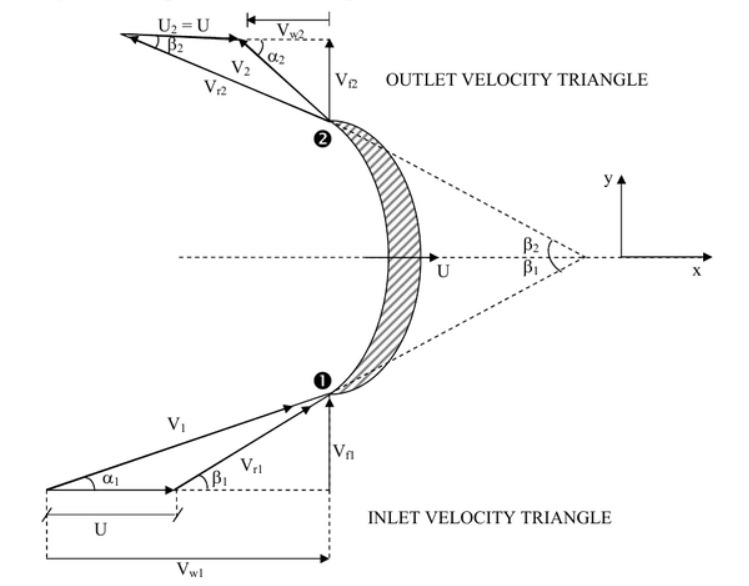
\includegraphics[width=0.8\textwidth]{img/curved_vane.jpeg} 
  \caption{Single moving plate / curved vane}
  \label{fig:curved_vane}
\end{figure} 

\begin{itemize}
  \item $v_1. v_2 \rightarrow $ Absolite velocities of the jet at inlet and outlet respectively
  \item $u_1, u_2 \rightarrow $ peripheral velocity of the vane at inlet and outlet respectively
  \item $v_{r1},v_{r2} \rightarrow $ relative velocity in inlet and outlet respectively.\\

  \begin{minipage}{0.20\textwidth}
    \begin{tcolorbox}[boxrule=1pt,width=\linewidth]
    $u + v_r = v$ \\
    $\Rightarrow v_r = v - u$ 
    \end{tcolorbox}
  \end{minipage}
  \begin{minipage}{0.33\textwidth}
    \begin{tcolorbox}[boxrule=1pt,width=\linewidth]
    $v_w, v_f$ is the components of $v$
    \end{tcolorbox}
  \end{minipage}

  \item $v_{f1}, v_{f2} \rightarrow $ velocity of flow at inlet and outlet respectively. alternatively, components of absolute velocity normal to the direction of motion.
  \item $v_{w1}, v_{w2} \rightarrow $ velocity of whirl at the inlet and outlet respectively. alternatively, components of absolute velocity in the direction of motion.  
\end{itemize}

\end{document}
